\title{Development of a Curved Layer Carbon Fiber 3D Printer}
\author{Jackie Song, Peter Ascoli}
\documentclass{article}
\usepackage[margin=1in]{geometry}
\usepackage[pdftex]{graphicx}
\usepackage{epstopdf}
%\usepackage[autolinebreaks]{mcode}
\usepackage[section]{placeins}
\usepackage{gensymb}
\usepackage{mathtools}
\usepackage{fancyhdr}
\pagestyle{fancy}
\lhead{Peter Ascoli \& Jackie Song}
\chead{ME163: Senior Project}
\rhead{\rightmark}
\renewcommand{\headrulewidth}{0.4pt}
\renewcommand{\footrulewidth}{0.4pt}
\usepackage[colorlinks=true]{hyperref}
\usepackage[all]{hypcap}
\providecommand{\e}[1]{\ensuremath{\times 10^{#1}}}

%REPORT REQUIREMENTS:
%
%1) Applies exceptional analytical skills and synthesis of knowledge at system design level
%2) Integrates concepts from different disciplines and recognizes applicability of concepts to design problem
%3) Clearly articulates design criteria and constraints
%4) Factors all constituents that contribute to design criteria and constraints and recognizes how design decisions impact design criteria and constraints
%5) Formulates clear problem statement
%6) Articulates problem solving process and outlines compelling strategy for finding quality solution
%7) Concise, well-organized and well-written
%8) Professional quality technical content
%9) Performs relevant and reputable literature review and demonstrates awareness of state-of-the-art

\begin{document}
\maketitle
\tableofcontents
\thispagestyle{plain}
\clearpage

\listoffigures
\listoftables

\clearpage

%----------------------------------------------------------
%\begin{abstract}

Current desktop 3D printers use FDM (Fused Deposition Modeling) to build parts out of flat layers of extruded thermoplastics. The printed parts have poor mechanical properties because of the low strength of thermoplastics and because the flat layer geometry limits inter-layer adhesion in thin areas. A curved-layer CFRP (Carbon Fiber Reinforced Polymer) 3D printer is being developed to solve those two issues. With curved layers, the carbon fiber may be oriented to best suit the applied loading on any given part, and the layers may be designed for greater inter-layer adhesion. An FDM-compatible ABS-matrix CFRP filament was developed and shown to have promising mechanical properties, comparable to aluminum. A custom FDM extruder was designed and prototyped for mounting on an available FANUC industrial robot arm, which provides the six necessary degrees of freedom to print curved layers. Control electronics were assembled and will be programmed to control the custom extruder and take input signals from the FANUC robot controller. A composite-specific finite element analysis software package was acquired and will be used to optimize the print layer geometry. Future work includes building the custom extruder; refining the filament production and test methods; programming the robot and extruder controller; generating optimized layer geometries; and printing and testing the CFRP material. 

\end{abstract}

%
%\clearpage

%----------------------------------------------------------
\section*{Nomenclature}

\begin{tabbing}

  XXXXXX \= \kill% this line sets tab stop

  $ABS$ \> Acrylonitrile Butadiene Styrene\\
  $PLA$ \> Polylactic Acid\\
  $FDM$ \> Fused Depostion Modeling\\
  $CFRP$ \> Carbon Fiber Reinforced Plastic, or Carbon Fiber Reinforced Polymer\\
  
\end{tabbing}


\clearpage


%----------------------------------------------------------
\section{Introduction}

\subsection{Problem Definition}

\indent

3D printing technologies offer the ability to produce new parts quickly, allowing faster and cheaper design iterations. However, commercially available Fused Deposition Modeling (FDM) 3D printers currently produce relatively weak parts due to the materials and print method used. They print using weak thermoplastics, most commonly polylactic acid (PLA) or acrylonitrile butadiene styrene (ABS), and deposit the material only in planar layers parallel to the build platform. Because of poor layer adhesion, this method yields parts that fail quickly under loading due to layers being sheared or pulled apart; this type of failure is particularly evident in parts with thin bosses or shells normal to the build plane, which offer very little surface area for layers to bond. Some parts may be rotated in the printer software to maximize layer contact area, but the planar layer limitation remains. These faults in FDM printers limit much of 3D printing to rapid prototyping applications (where strength is not necessary) despite high demand for printers that can produce stronger parts for use in load-bearing applications. Subsequently, there exists a need for 3D printers using alternative materials and layer formulations that are capable of printing more usable parts.\\

\subsection{Background Research}

\indent

sample text

\subsection{Project Approach}

\indent

To create stronger 3D printed parts we are developing a Curved Layer Carbon Fiber 3D Printer. The printer will utilize FDM techniques to deposit one continuous strand of a carbon fiber reinforced plastic (CFRP) filament in curved layers. This material will mirror existing, widely used fiber-reinforced polymer materials, such as carbon fiber and fiberglass composites. Using curved layers will orient fibers in optimal direction(s) for withstanding applied loads.

To realize the goal of a fiber-reinforced composite curved layer 3D printer, the project was broken down into five subsystem, which are outlined in Figure.

%We intend to create stronger 3D printed parts by build	ing a printer capable of depositing a continuous strand of fiber-reinforced polymer in curved layers. The material will mirror existing, widely used fiber-reinforced polymer materials, such as carbon fiber and fiberglass composites. Using a serial robot arm instead of a typical cartesian coordinate robot will allow the printer to lay material in any direction. Freedom from the planar layer limitation, combined with precise control over toolpaths, will allow the fibers to be oriented optimally for the desired mechanical properties of the part. These properties will be user-determined based on expected loading, surface finish, or other requirements. Experimental comparisons between curved layer FDM and standard FDM parts will quantify the increase in strength and provide insight towards op- timizing fiber orientation.\\
%
%To realize the goal of a fiber-reinforced composite curved layer 3D printer, we will first learn to use to the FANUC LR Mate 200iC robot in The Cooper Union’s ME Rapid Prototyping Lab. This robot arm provides the necessary degrees of freedom for curved layer printing. We first plan to familiarize ourselves with the arm and control software by developing tool paths within its operational envelope. Then, we can mount an extruder to the arm and use an existing software toolchain to create standard flat-layer thermoplastic FDM prints. Once the standard print method is implemented, we can implement new gcode to create curved layer thermoplastic prints, while simultaneously investigating the best fiber composite to use as printing material. We will then alter the extruder mechanism to work with the chosen material. Finally, with curved layer fiber-reinforced 3D printing achieved, we plan to experimentally compare the mechanical strength of curved layer fiver-reinforced FDM prints to thermoplastic flat-layer FDM prints; the Instron machine in The Cooper Union’s ME Materials Lab can be used to load the parts and strain gauges can be attached to the parts to monitor specific local stresses.

%problem definition, background research, our project goal(s)

\clearpage

%----------------------------------------------------------
\section{3D Printing Toolchain}

\subsection{Extruder}

\indent

The extruder is the mechanism responsible for depositing the filament in a 3D printing system. Generally, this mechanism includes a motor that drives a gripping mechanism, which reels in and pushes the filament into a heated nozzle. The nozzle heats the filament to a soft state and lays the filament on the printing bed or on an already printed layer to create the part.\\

In the case of the curved layer carbon fiber 3D printer, the extruder is required to mount to the robot arm, be compact\footnote{The compact size is required for two reasons. First, to ensure that induced torque on the robot arm joints and gripper remain within safe operating conditions. Second, to readily permit the nozzle to deposit material when not perpendicular to the build platform, which will be required for printing curved layers.}, and accept filaments of a variety of sizes (likely ranging in diameter from 1.75 mm to 3 mm). \\

Figure~\ref{fig:old extruder} presents the initial design of the extruder in \emph{SolidWorks}. The extruder mounts to the Fanuc grippers and is constructed out of a combination of machined aluminum parts and RepRap hardware (nozzle, J-head, J-head mounting plate, ceramic heating element, thermistor, fan, and fan mount). This configuration locates the nozzle outlet along the mid-plane of the grippers for simple coordinate transformations when programming the robot to print. Laser-cut acrylic gears provide a 3:1 step up in torque from the stepper motor and drive a notched screw, which grips and pushes the filament into the nozzle. A bearing opposite the screw provides counter-pressure and its mounting plates can adjust the distance between the screw and bearing to accommodate different filament sizes.\\

\begin{figure}[h!]
\centering
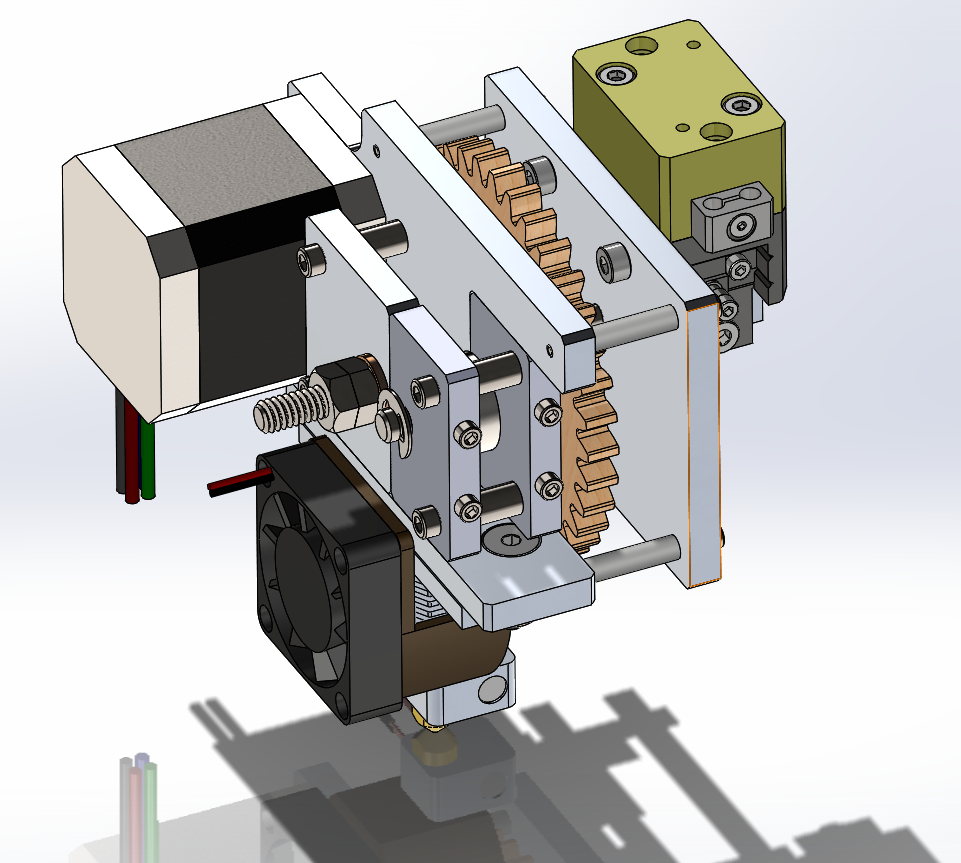
\includegraphics[width=0.5\textwidth]{./figures/extruder-old-2}
\caption{An isometric view of the initial extruder design.}
\label{fig:old extruder}
\end{figure}

To assess the feasibility of the initial extruder design, minor tweaks were implemented within the CAD to make a laser-cut prototype.  Figure~\ref{fig:prototype extruder} shows the prototype mounted on the FANUC grippers. The prototype served its purpose and demonstrated numerous problems with the initial design. There were some mis-measurements of RepRap hardware, using spacers instead of threaded standoffs decreased the rigidity of the structure, the structure was a bit larger than desired, and a few undetected interferences were discovered. Subsequently, the extruder then went through a series of redesigns to develop an acceptable configuration.\\

\begin{figure}[h!]
\centering
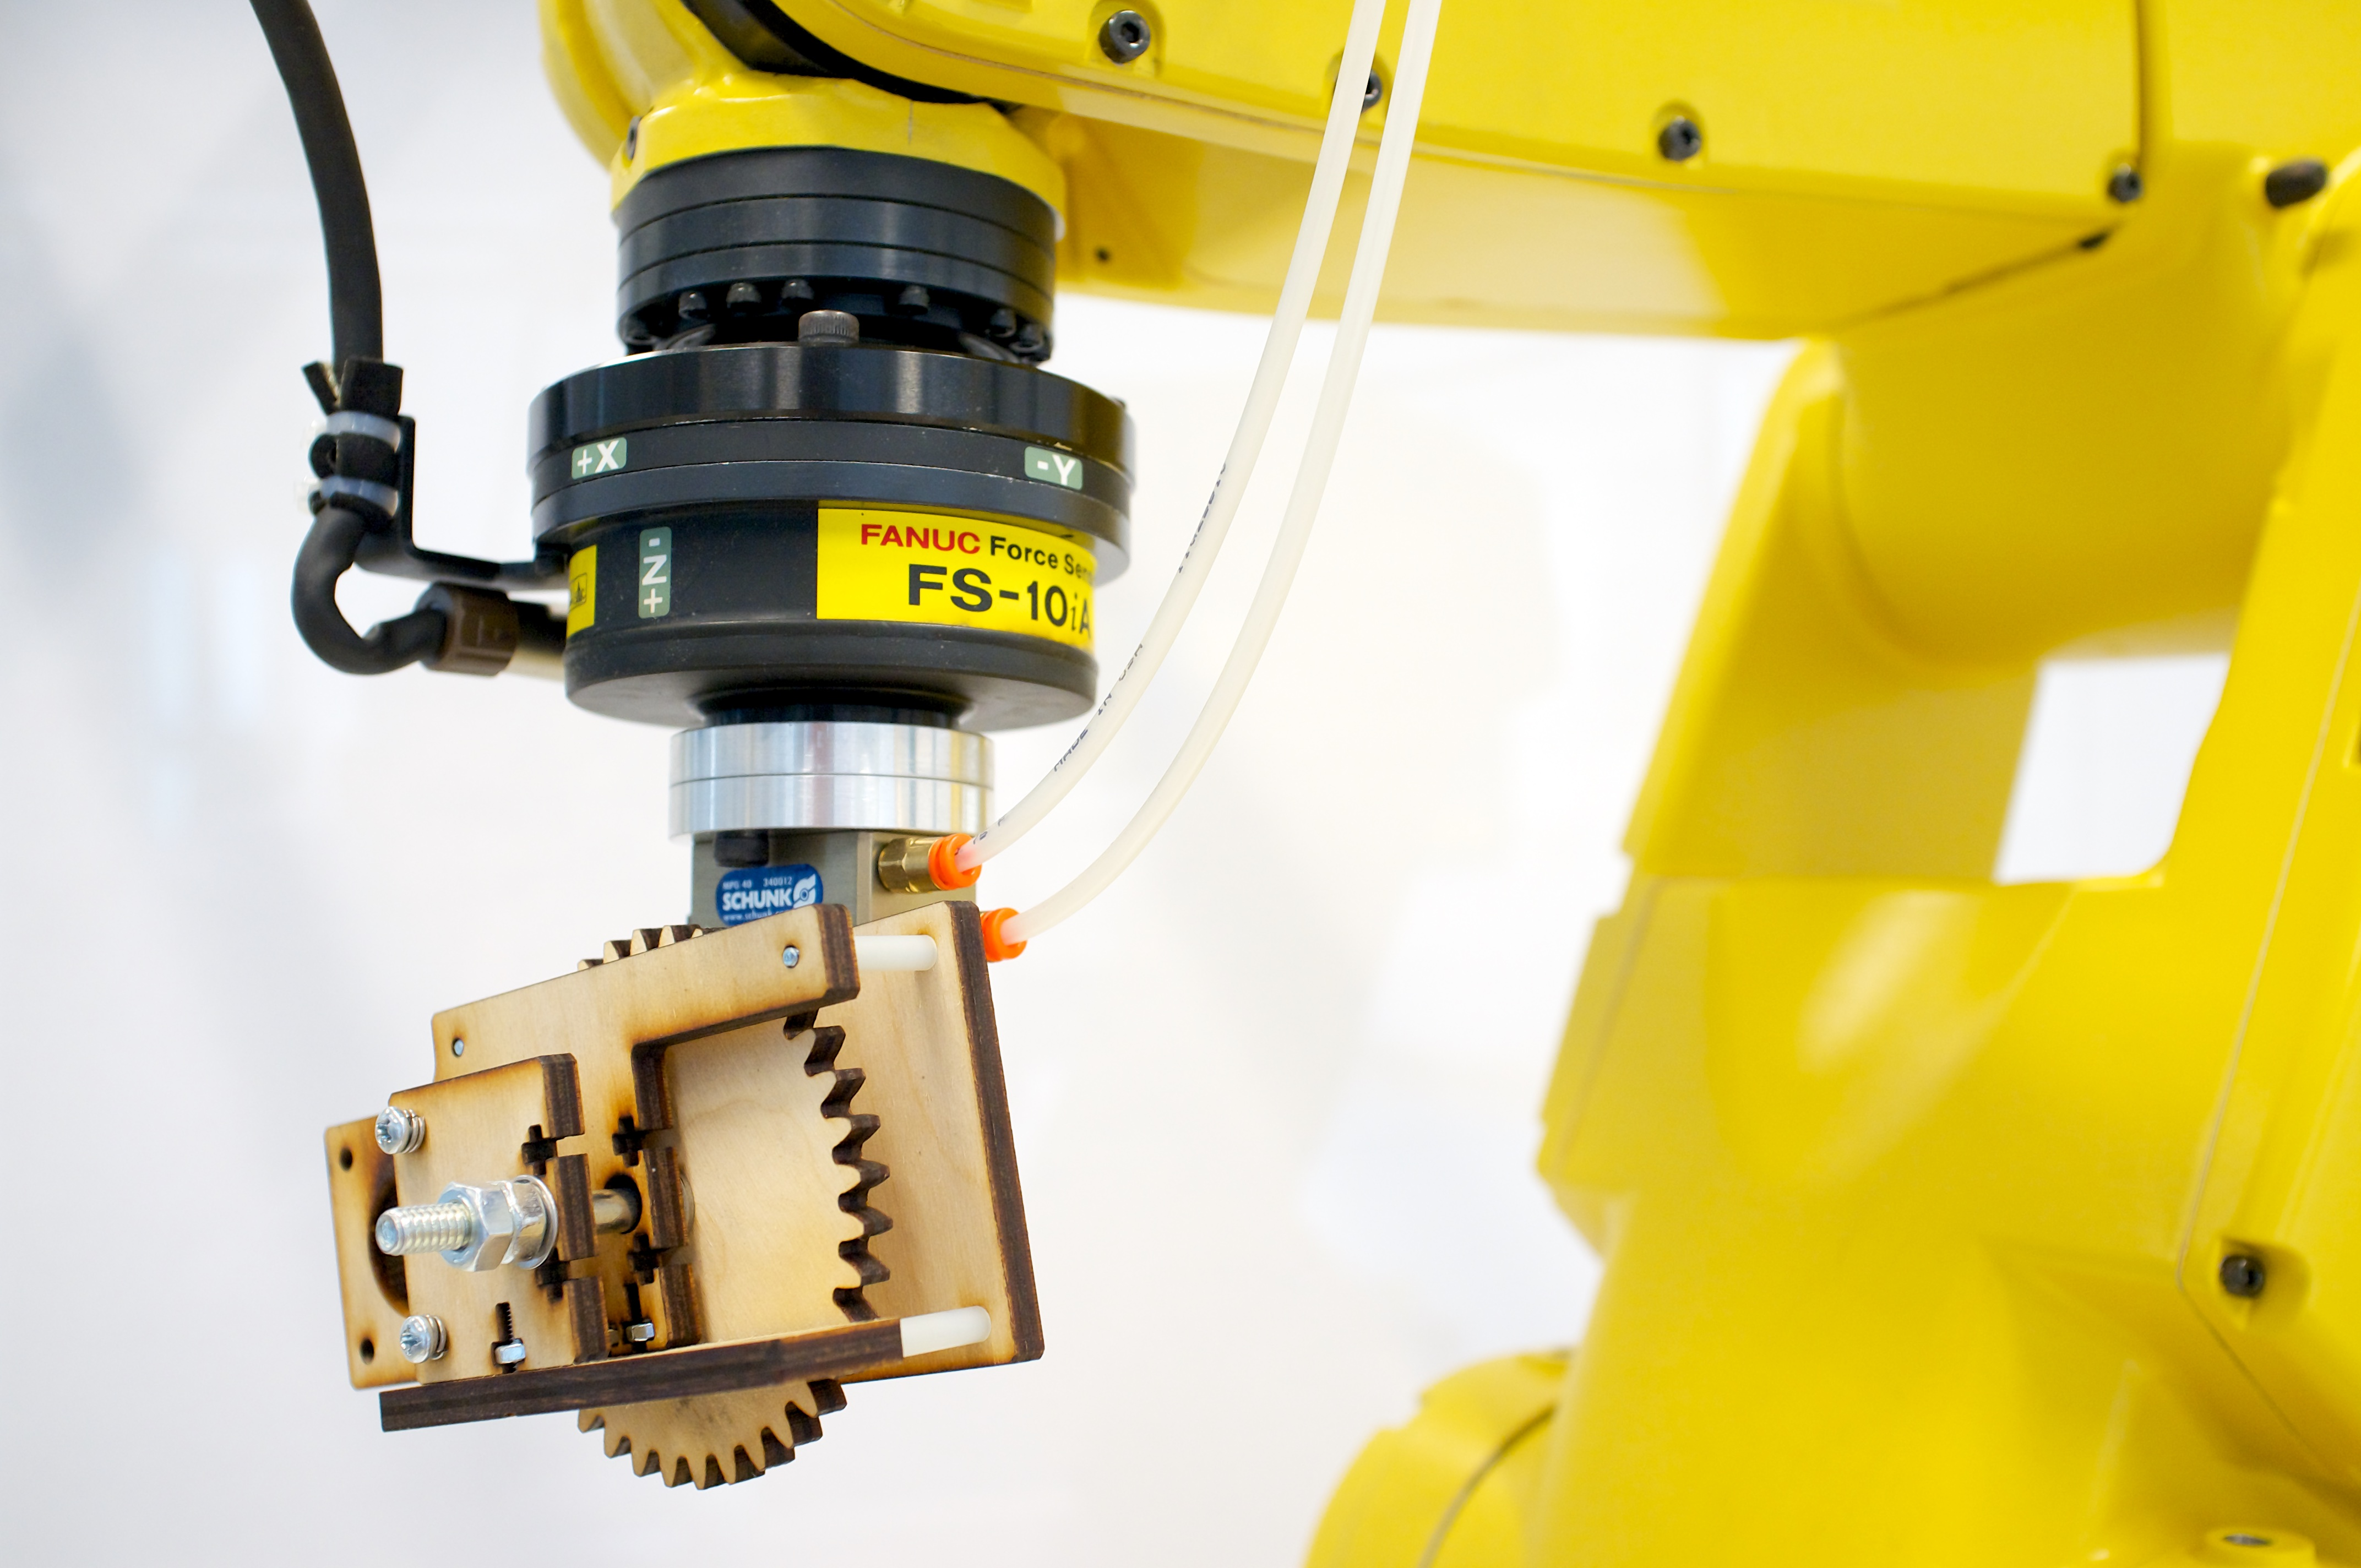
\includegraphics[width=0.5\textwidth]{./figures/extruder-prototype-2}
\caption{A photograph of the mounted prototype.}
\label{fig:prototype extruder}
\end{figure}

Figure~\ref{fig:extruder iso} presents a rendering of the final extruder design. Figure~\ref{fig:extruder drawing} provides general dimensions and annotations to fully present the extruder design concept. The final design is significantly smaller than the initial design, will require less machining, and uses less fastening hardware. The size decrease was accomplished by using smaller gears (50\% scaled versions of gears dimensions taken from \emph{SDP-SI}\footnote{\url{http://www.sdp-si.com/}} and located the stepper motor directly beneath the FANUC grippers. As part of the design process the gears were laser-cut, and physically tested to ensure that the teeth would not shear off under a load less than the stall torque of the stepper motor, before being fully committed to this design. The stepper motor (Sparkfun ROB-10846) outputs 68 oz-in of torque and has a resolution of 400 steps/revolution. Two laser-cut acrylic gears step up the torque to 204 oz-in.\footnote{Most extruders in the 3D printing community use analogous stepper motors and utilize gear trains to step up the torque. Common gear ratios range from 2:1 to 4:1 depending on the specific qualities of the filament. Given that the specifics of the filament are not yet fully determined, the mean value was used.} A partially threaded screw will be notched on the mill to contain teeth-like features along a portion of its length. These teeth will grip the filament and push it into the extruder. The screw rides along two bronze PTFE-coated bearings to ensure smooth rotation during printing. Two adjustment plates locate a bearing just opposite the screw to provide counter-pressure during printing. The plates are secured in place using four screws, which can be loosened or tightened to adjust the distance between the screw and bearing to accommodate different filament sizes. Shims or spring washers may have to be utilized to located this adjustable mechanism in its optimal position for the official CFRP.\\

The extruder will be machined with aluminum to provide rigidity. Many 3D printers utilize 3D printed bodies for mounting RepRap hardware, but the associated poor tolerances and material flexibility are not ideal for the curved layer carbon fiber 3D printer. Machining the extruder out of aluminum will allow easy implementation of any future adjustments and ensures all mechanisms will align properly. The entire extruder assembly secures to the FANUC gripper with four screws.\\

\begin{figure}[h!]
\centering
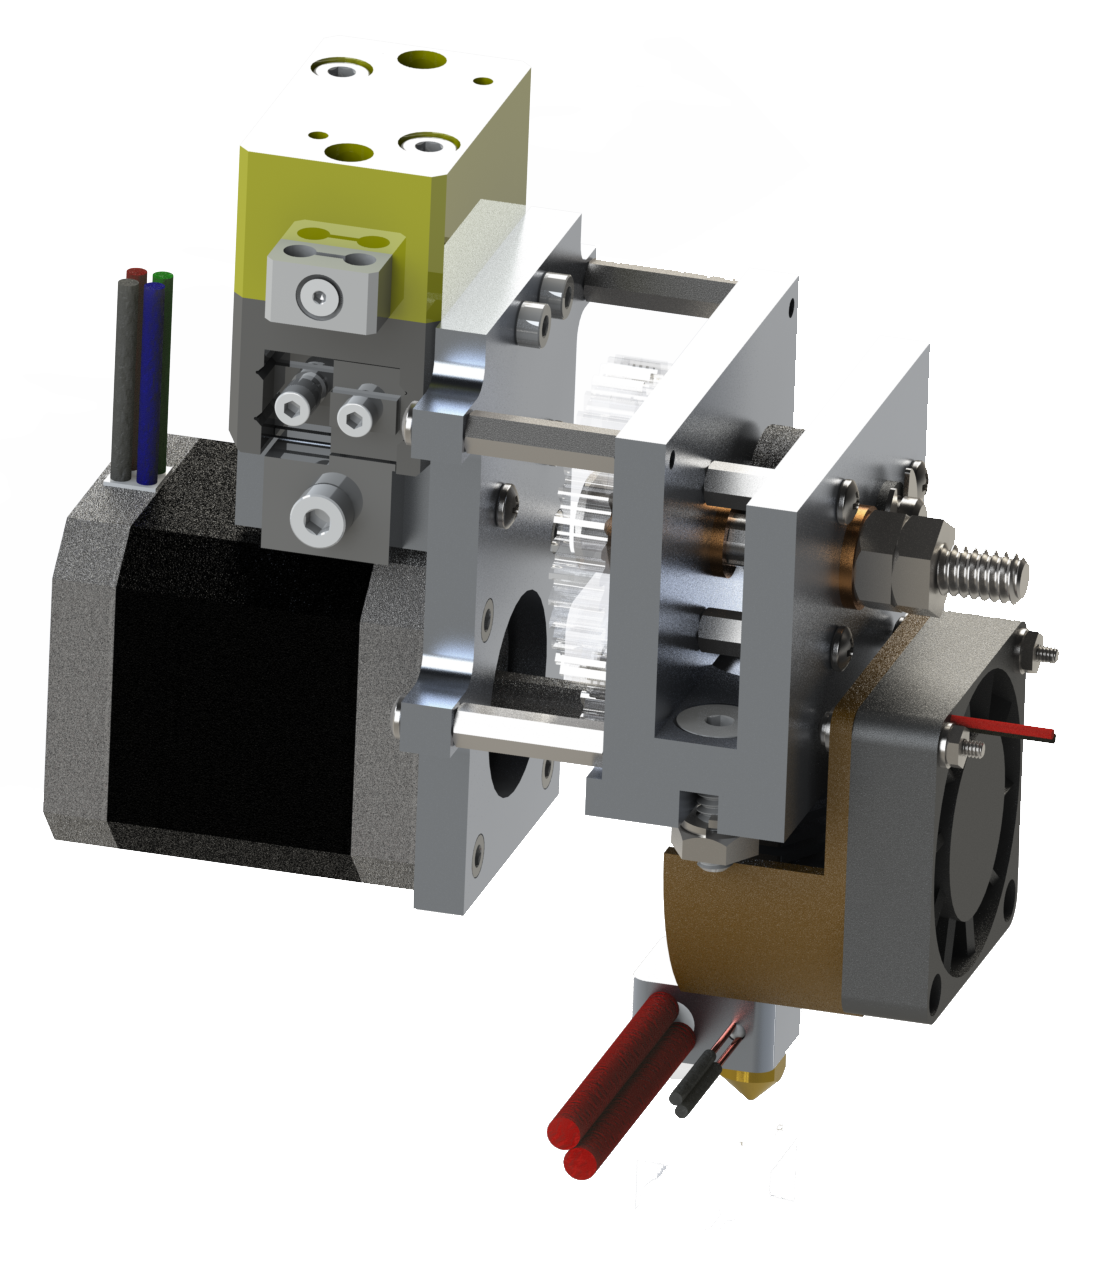
\includegraphics[width=0.5\textwidth]{./figures/extruder-iso}
\caption{An isometric render of the final extruder design.}
\label{fig:extruder iso}
\end{figure}

\begin{figure}[h!]
\centering
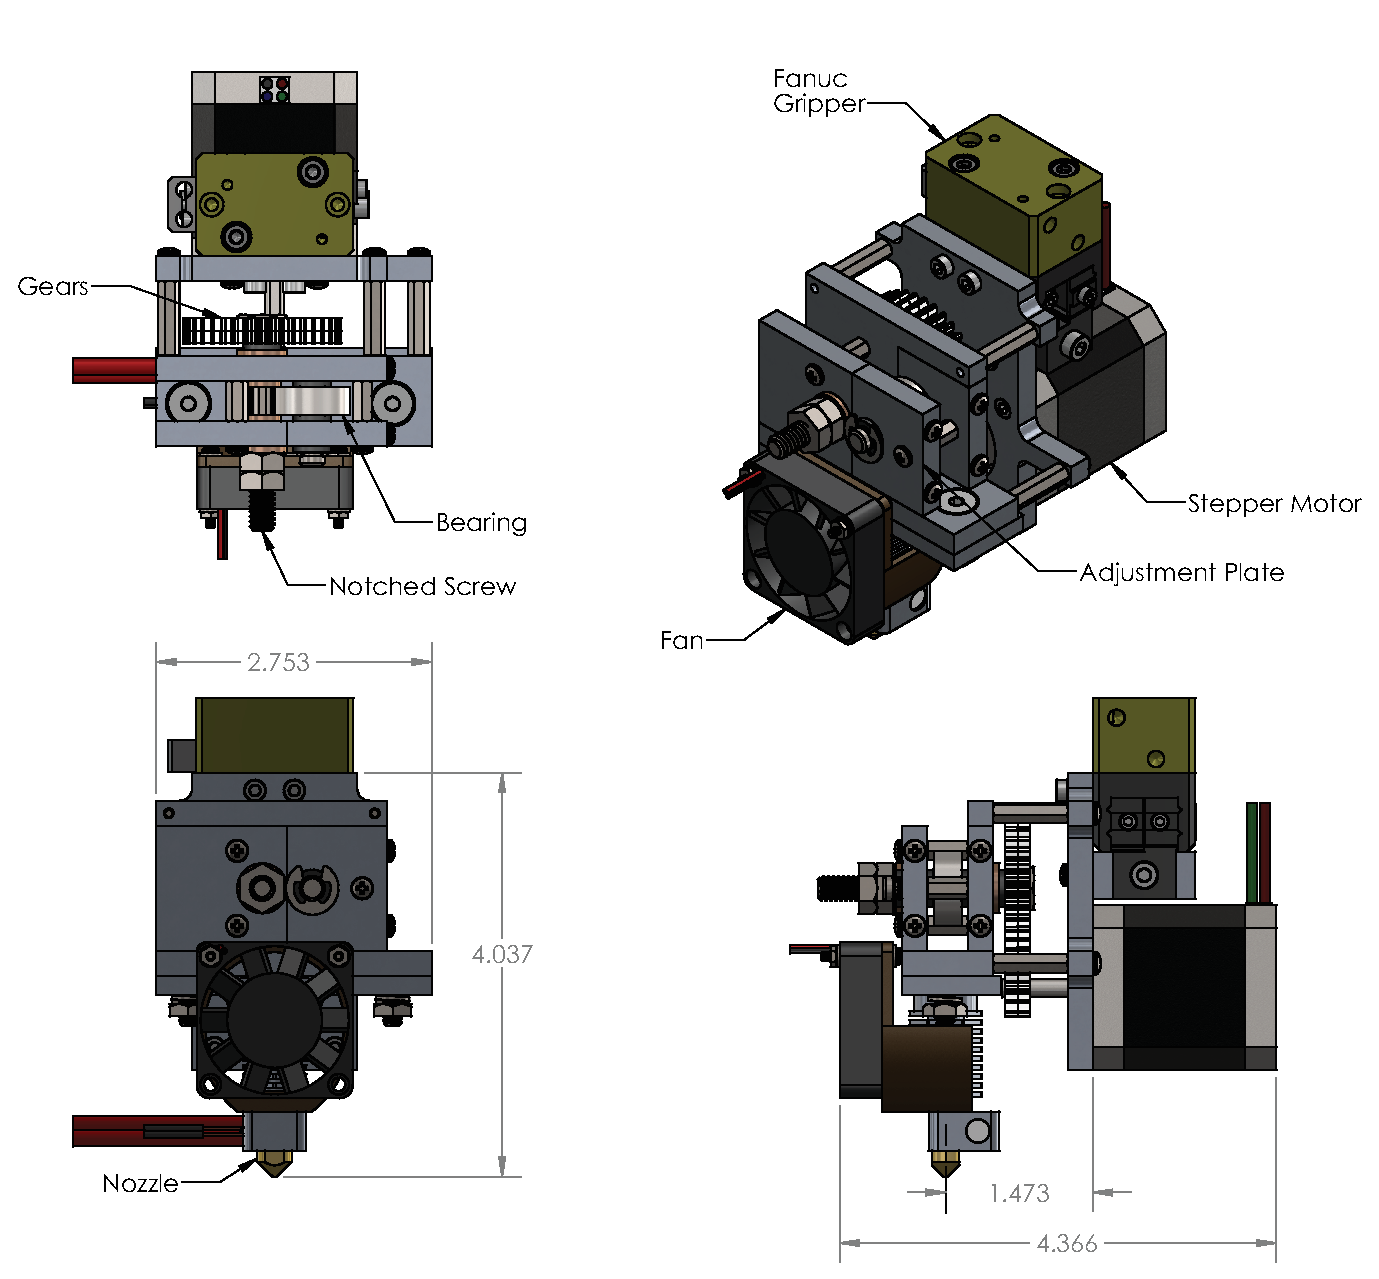
\includegraphics[width=1\textwidth]{./figures/extruder-drawing}
\caption{A general drawing of the final extruder design.}
\label{fig:extruder drawing}
\end{figure}

\clearpage




\subsection{Control Electronics}

\indent 

The extruder is controlled by a Megatronics control board, shown in Figure~\ref{fig:megatronics}, which was developed for the RepRap open source 3D printer project. The board contains all the necessary electronics to drive a Cartesian coordinate based FDM desktop 3D printer. The board can drive numerous positioning and extruder motors, heating elements, sensors, displays, and more. Because the FANUC robot handles the extruder positioning, the Megatronics board will be used to control the extruder elements only.\\

\begin{figure}[htp]
\centering
\includegraphics[width=0.5\textwidth]{./figures/electronics-board}
\caption{A photo of the Megatronics Control Board.}
\label{fig:megatronics}
\end{figure}

\subsubsection{Firmware}

\indent

When used in RepRap printers, the Megatronics board is typically used with one of several open source firmwares that are also associated with the RepRap project. Because these firmwares were designed with Cartesian desktop FDM printers in mind, they work well with the Megatronics board. The chosen firmware is uploaded to the board using a USB cable. For the FANUC-mounted extruder, a suitable firmware will be chosen and modified to work with the FANUC robot.\\

The firmware will be modified to control only the components present on the FANUC-mounted extruder. The firmware's timing functions must be modified as well. Normally, the firmware calculates its own filament feed rates and motor speeds in order to ensure that the flow rate of the extruded material follows the surface speed of the extruder with respect to the print surface. Because the FANUC controller has its own closed-loop control and is much less flexible than the RepRap firmware, the firmware will be modified to monitor the FANUC robot speed and position, and act accordingly. The monitoring will be accomplished by polling robot status system variables from the FANUC controller.

\subsubsection{Enclosure}

\indent

The Megatronics board is too large to be mounted directly to the extruder, so it has been mounted inside the FANUC robot cage. The board is housed in a clear acrylic housing, shown in Figures~\ref{fig:megatronics-mount-back} and \ref{fig:megatronics-mount-front}, which serves several purposes. The housing protects the board from debris and accidental touches by either people or by the robot. The clear front makes the on-board status LEDs visible for debugging and operation. The back of the housing has built-in slots that provide anchors for cable management hardware. The cable management hardware will both organize the wires connected to the board and provide strain relief. The strain relief is especially important for the wires that connect the board and the extruder, because they will move with the extruder. The housing is positioned in a location that will cause the least interference between the wires and the arm. The power and USB cables for the board will be routed through the robot cage members. The USB cable will provide convenient access for updating the board firmware and collecting data using a laptop. 

\begin{figure}[htp]
\centering
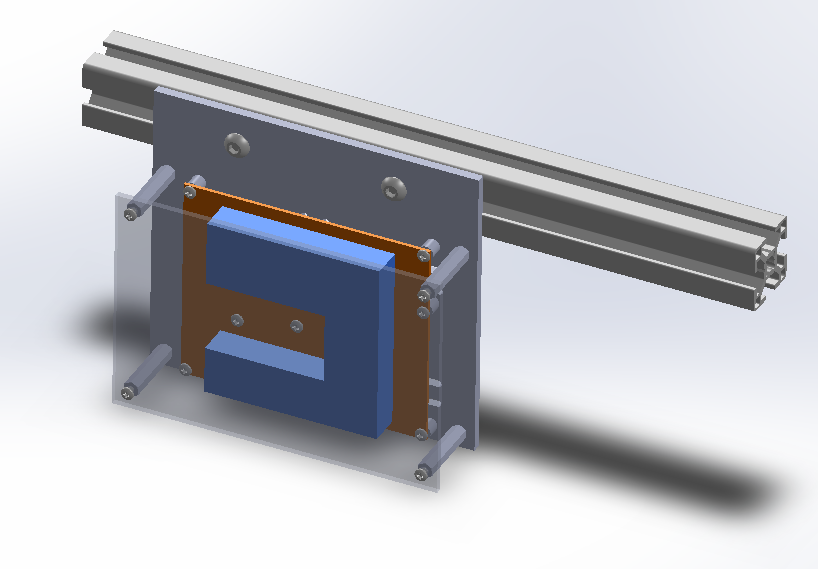
\includegraphics[width=0.5\textwidth]{./figures/megatronics-mount-1}
\caption{A \emph{SolidWorks} model of the mounted Megatronics board.}
\label{fig:megatronics-mount-back}
\end{figure}

\begin{figure}[htp]
\centering
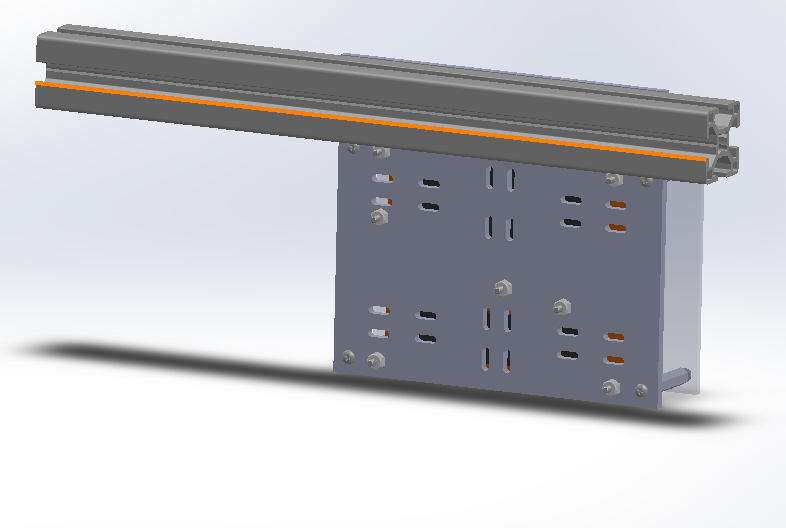
\includegraphics[width=0.5\textwidth]{./figures/megatronics-mount-2}
\caption{A \emph{SolidWorks} model of the mounted Megatronics board.}
\label{fig:megatronics-mount-front}
\end{figure}




%extruder, control electronics, slicing algorithm & layer generation

\clearpage

%----------------------------------------------------------
\section{6 Degree of Freedom Manipulator}

To extrude a consistent bead of material along a surface, the extruder nozzle should be normal to the surface. This means that in flat layer printing, the extruder may always be held vertically above the print surface. However, curved layers may require the extruder to tilt and rotate to reach some areas properly. Thus, curved layer FDM 3D printing requires the extruder positioning mechanism to have more degrees of freedom than flat-layer printing. 

The FANUC LR Mate 200iC 6 degree of freedom industrial robot arm provides the necessary degrees of freedom for curved layer printing. The robot was acquired as part of an eductional package that includes the robot, its housing, the controller, a gripper and vision system, and related softwrae. The robot is compact and has positioning repeatable to .02mm. As such, the robot is a suitable platform for a curved layer 3D printer. The extruder will be mounted to the existing gripper, and the control electronics and filament will be mounted to the side of the robot cage.


%robots

\clearpage

%----------------------------------------------------------
\section{Carbon Fiber Filament}

\indent

In order to print the CFRP material, the carbon fiber and resin will be combined into a CFRP filament. As in conventional FDM printing, the CFRP filament will be extruded by driving it through a heated nozzle. ABS plastic was chosen as the matrix material for this filament for several reasons. First, ABS has already successfully been combined with chopped carbon fiber in FDM filaments. Second, ABS does not require post-processing to reach full strength, as epoxy-based pre-impregnated carbon fiber composites do. In both filament development methods a 1K carbon fiber tow (shown in Figure~\ref{fig:carbonf-fiber-spool}) was utilized.\\

\begin{figure}[htp]
    \centering
    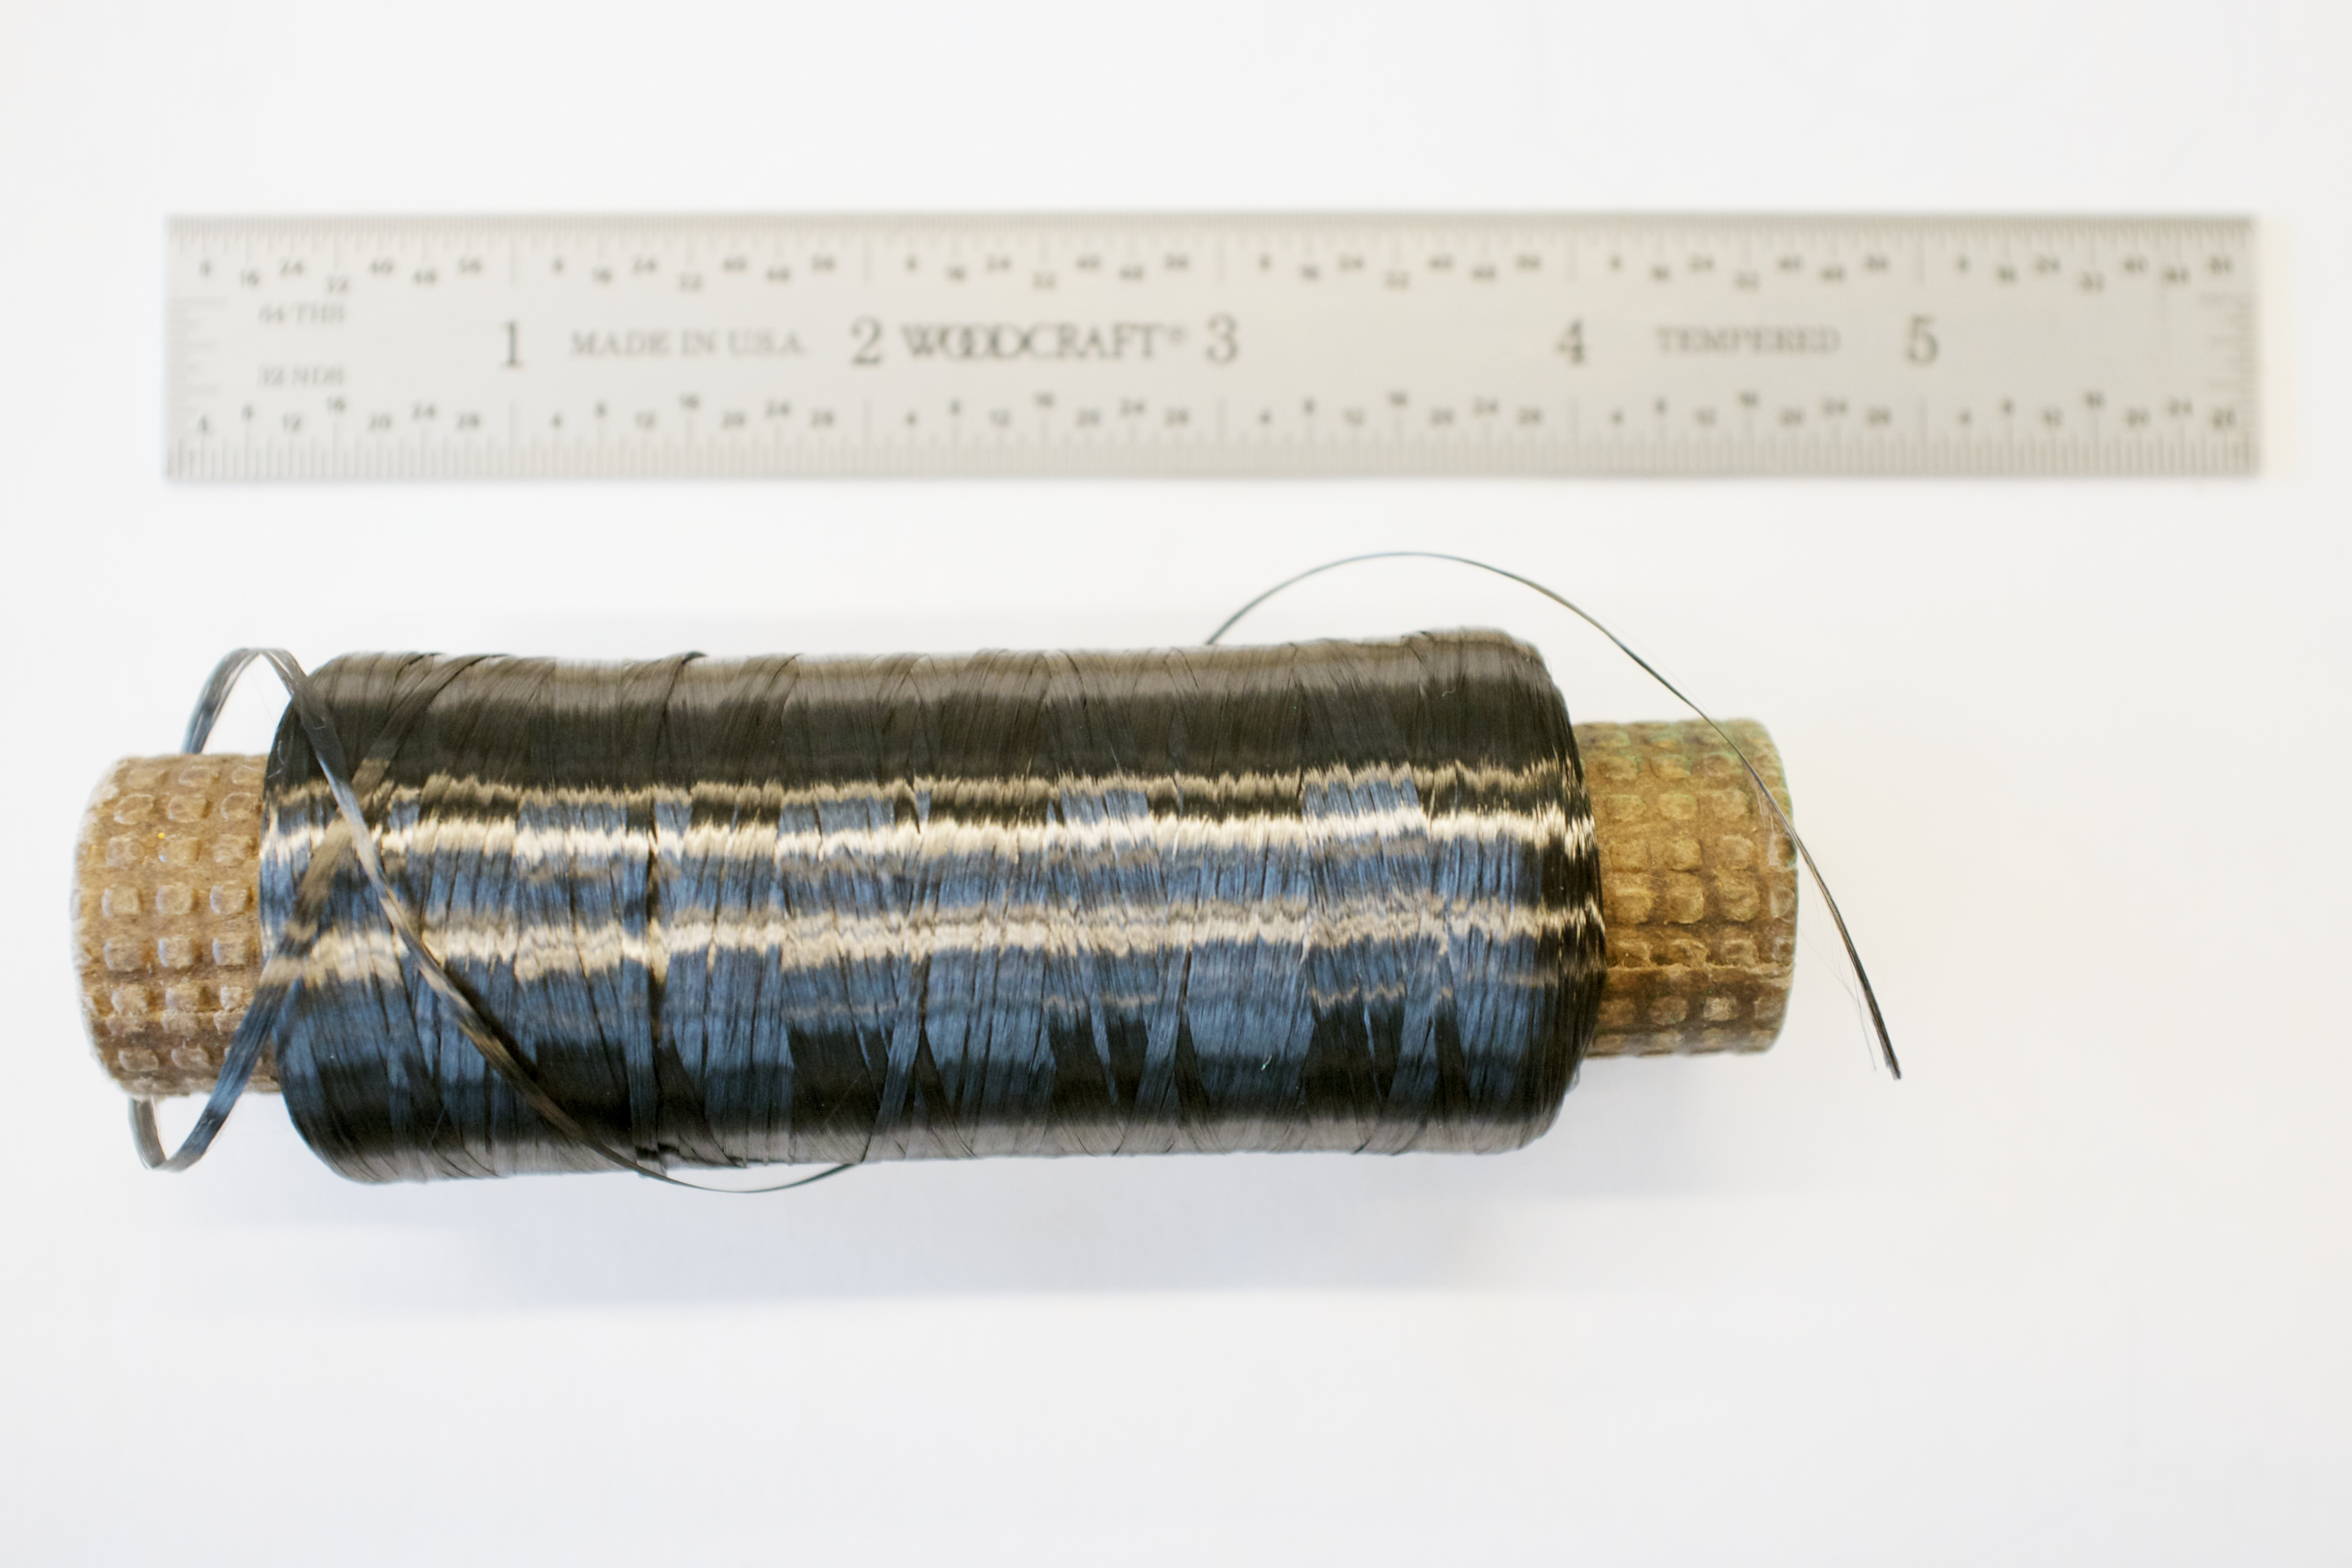
\includegraphics[width=0.5\textwidth]{./figures/carbon-fiber-spool}
    \caption{The 1K carbon fiber spool.}
    \label{fig:carbon-fiber-spool}
\end{figure}

\subsection{Production Methods}

\indent

Two production methods have been explored so far in the development of the CFRP filament. The first is pultrusion, a fabrication method widely used to manufacture fiber-reinforced structural members. A 3Doodler handheld 3D printing device was employed in pultrusion tests. The 3Doodler's feed motor was disabled, and then a bundle of carbon fiber and an ABS rod were simultaneously fed through the 3Doodler's heater and nozzle. The combined materials were manually drawn through from the exit end of the nozzle. This process is shown in Figure~\ref{fig:pultrusion-vid}. In the resulting filament, the carbon fiber bundle and the ABS adhered together well. However, due to the high viscosity of the heated ABS, most of the individual carbon fibers were not in contact with the ABS. This effect is visible in Figure~\ref{fig:pultruded-scope}.\\

\begin{figure}[htp]
    \centering
    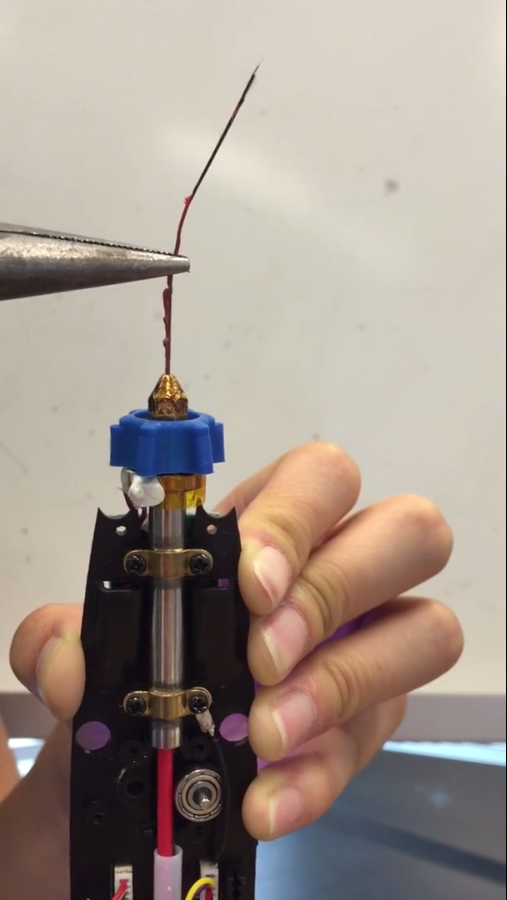
\includegraphics[width=0.4\textwidth]{./figures/pultrusion-vid}
    \caption{The experimental pultrusion setup, using the 3Doodler.}
    \label{fig:pultrusion-vid}
\end{figure}

\begin{figure}[htp]
    \centering
    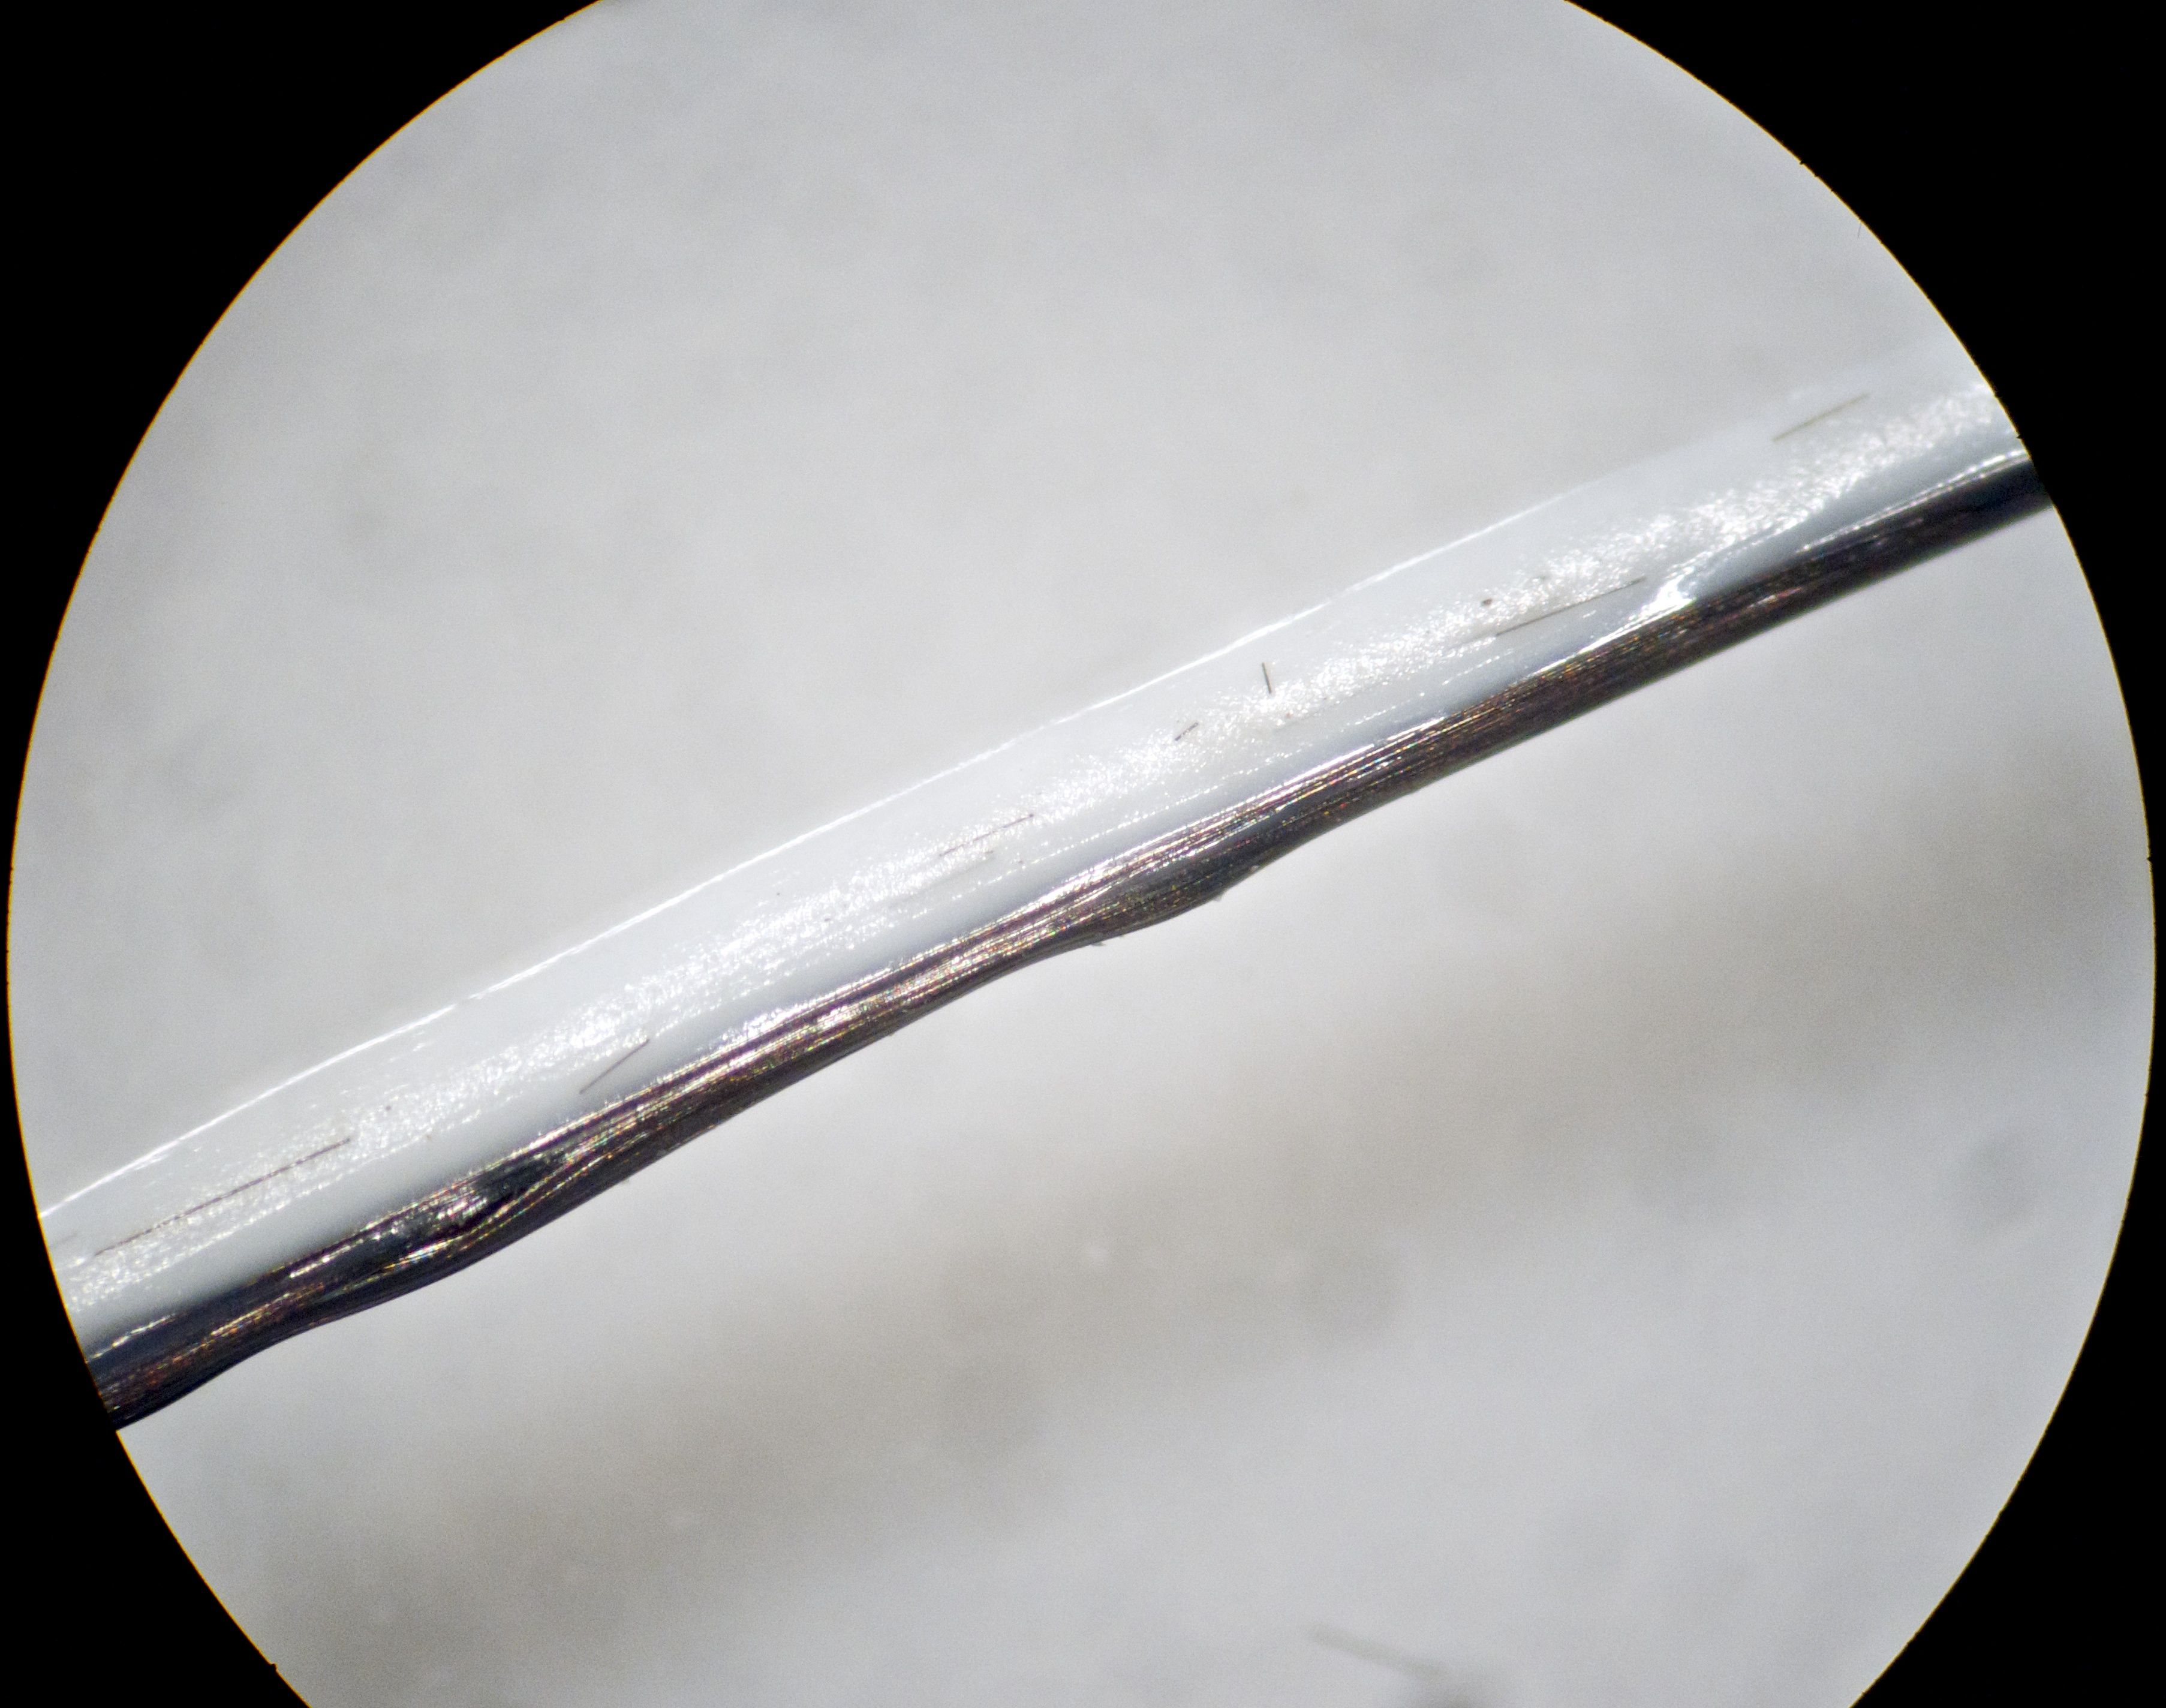
\includegraphics[width=0.6\textwidth]{./figures/pultruded-scope}
    \caption{Pultruded filament sample, magnified 10x under a microscope.}
    \label{fig:pultruded-scope}
\end{figure}

Good fiber wet-out is critical to the performance of fiber composites, so another filament production method was explored. In the new procedure, achieving complete wet-out was prioritized. ABS plastic was dissolved in acetone to make a thin slurry. A fiber guide was fabricated to guide the carbon fiber in and out of the slurry. Carbon fiber bundles were then drawn through the fiber guide and allowed to dry. The process setup is shown in Figure~\ref{fig:dipping-vid}. As the acetone evaporated from the slurry, a small amount of ABS was left on the carbon fibers. The resulting filament showed very good wet-out. A pultruded sample and a dipped sample are shown side-by-side in Figure~\ref{fig:two-samples}.\\

\begin{figure}[htp]
    \centering
    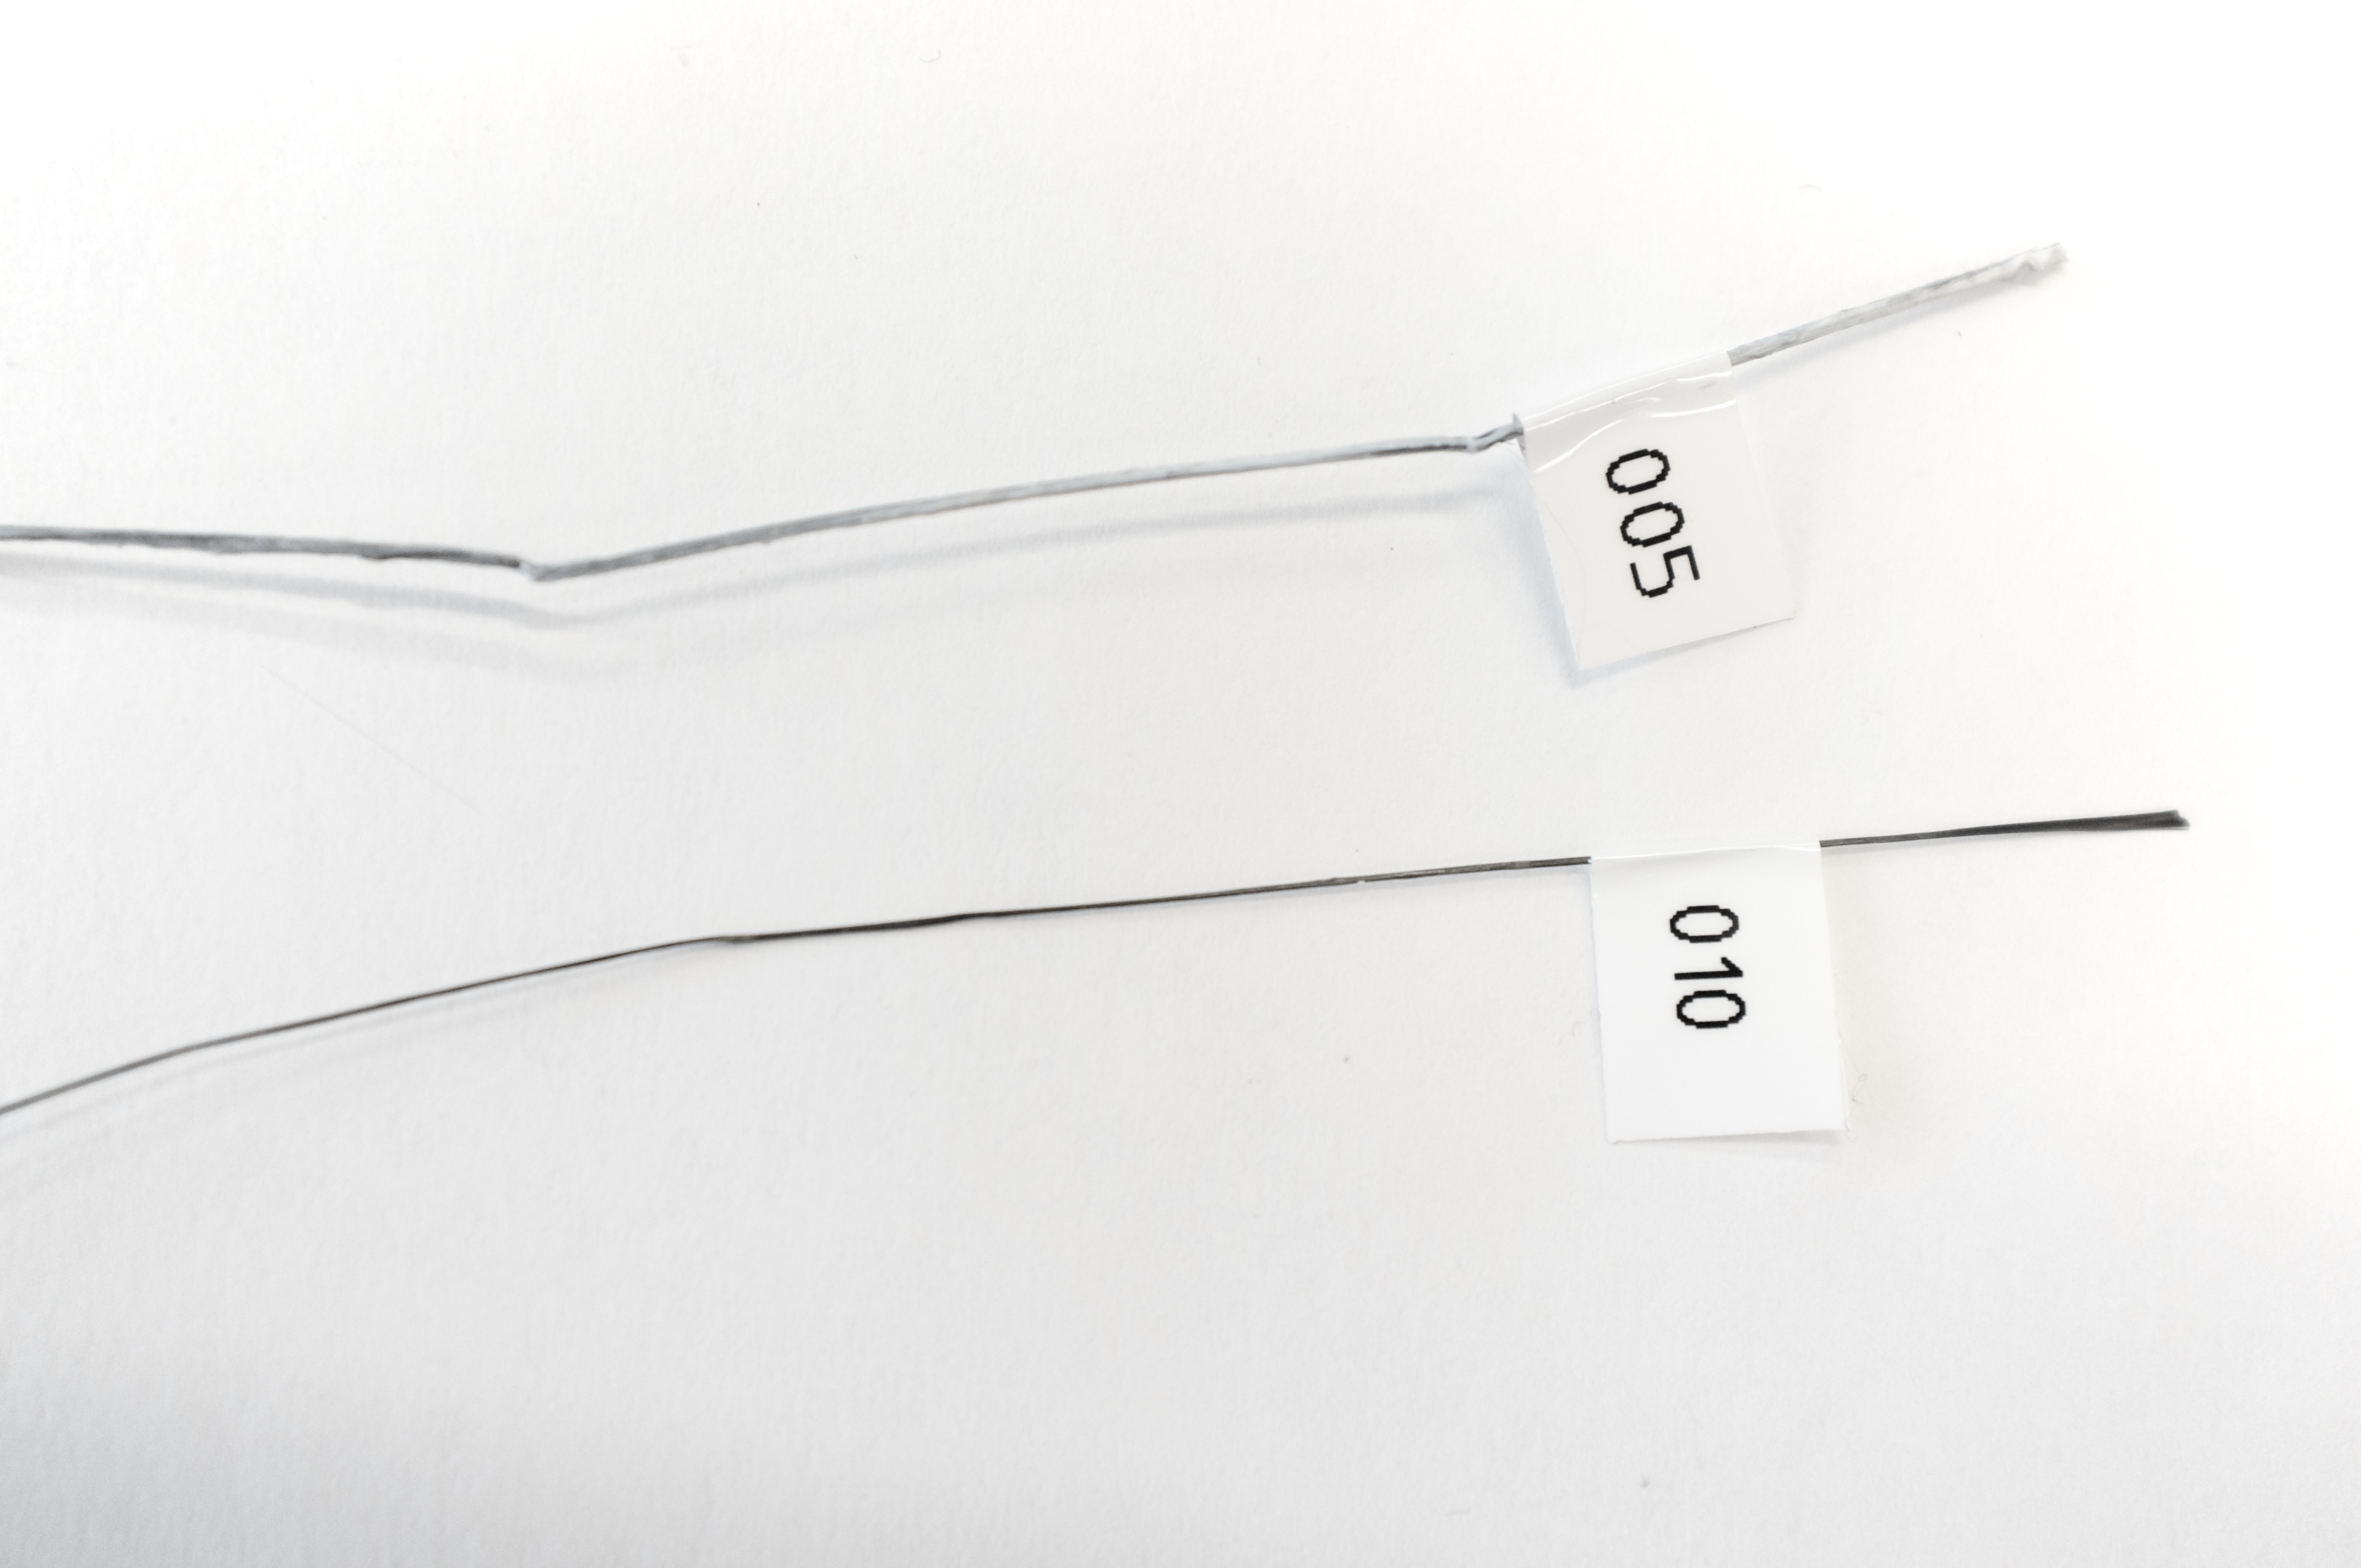
\includegraphics[width=0.6\textwidth]{./figures/FilamentSample}
    \caption{A pultruded filament sample (top) and a dipped filament sample (bottom), labeled with sample numbers.}
    \label{fig:two-samples}
\end{figure}

\begin{figure}[htp]
    \centering
    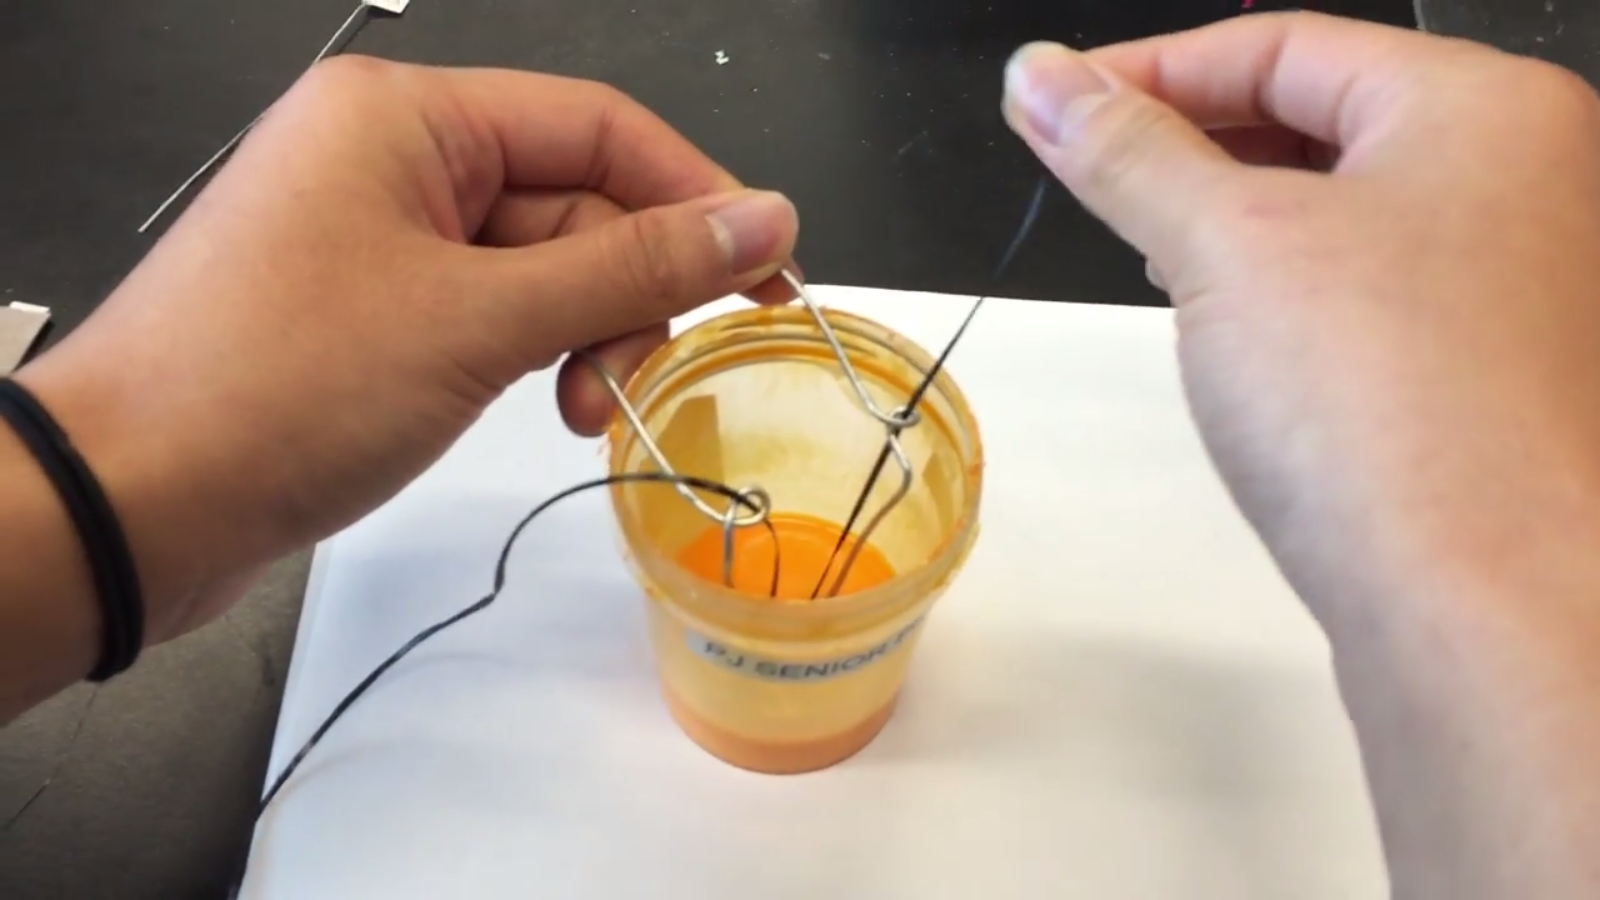
\includegraphics[width=0.8\textwidth]{./figures/dipping-vid}
    \caption{The basic slurry dipping process.}
    \label{fig:dipping-vid}
\end{figure}

\subsection{Mechanical Testing Setup}

\indent

Tensile tests were performed on the filament samples that were produced using the pultrusion and dipping methods. An Instron mechanical testing machine was used for these tests. Short lengths of filament (roughly 2 in) were cut from larger samples for testing. Due to the small, slippery,  and flexible nature of the filament samples, the regular serrated jaw inserts of the Instron tensile test jaws could not be used alone to secure the samples. Instead of clamping the samples directly in the jaws, the samples were securely mounted to aperture cards using melted ABS. The ends of the card were folded over the filament. Once clamped in the serrated jaws, the cardboard protected the filament from the jaws and held it securely in place. The card also assisted in aligning the filament with the jaws. Once clamped, the portion of the card was cut with scissors, and the test was started.\\

\subsection{Mechanical Testing Results}

\indent

The tensile tests performed on the filament samples provide insight into some of their basic mechanical properties. A representative tensile test data chart is provided in Figure~\ref{fig:instron-sample}. The CFRP samples showed fairly linear behavior before failing. Table~\ref{tab:test-results} compares the estimated ultimate tensile strength, stiffness, and density of two\footnote{Nearly a dozen samples were created. These two filaments selected for the table exhibited the most reasonable properties.} filament samples with those of ABS, carbon fiber, and aluminum 6061. The properties of aluminum were included for comparison because CFRP materials are often used to replace aluminum parts. Because it was difficult to consistently clamp the test samples without slipping once the test began, these are only very preliminary results. The results are also affected by inconsistencies in the filament samples themselves. Once the filament production method and test setup are further refined for consistency, further tests will be done to better characterize the properties of the filament. For now, however, the results are promising: both the pultruded and dipped filament samples are lighter and have a higher ultimate tensile strength than aluminum 6061, although they are not as stiff.\\

\begin{figure}[htp]
    \centering
    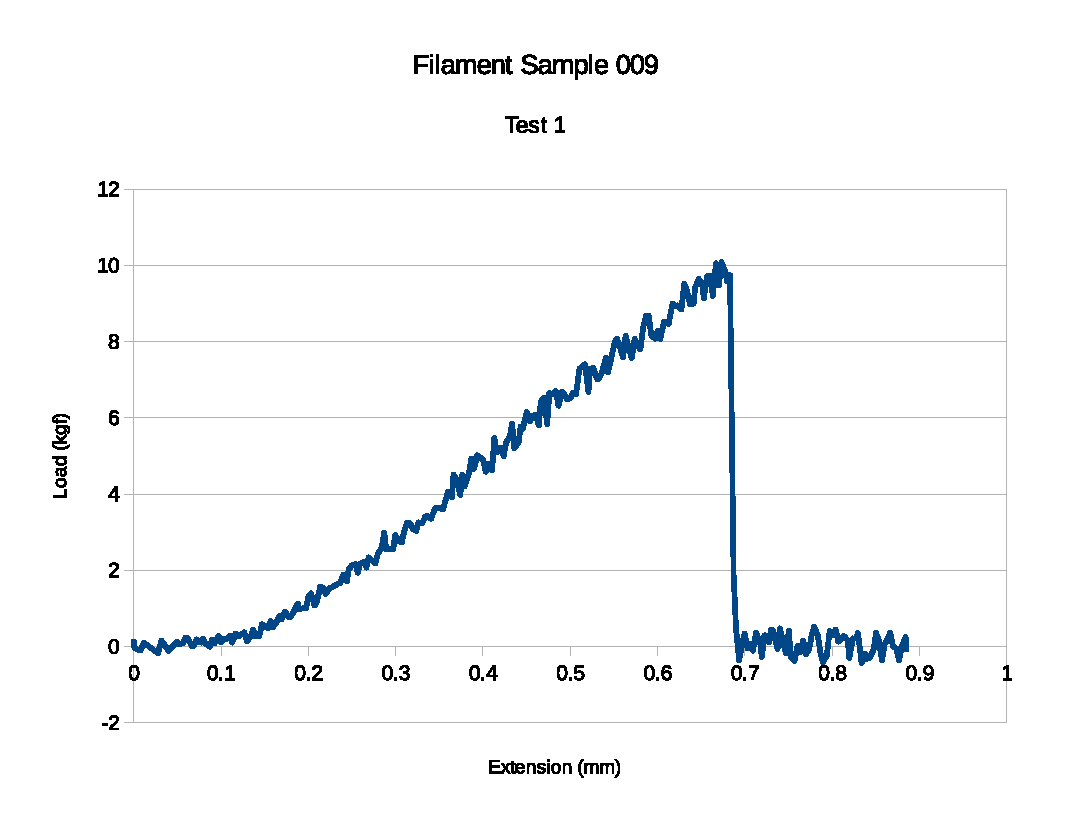
\includegraphics[width=0.8\textwidth]{./figures/009T1-instron-data}
    \caption{Sample tensile test data for a slurry-dipped filament sample.}
    \label{fig:instron-sample}
\end{figure}

\begin{table}[h]
    \centering
    \begin{tabular}{lcccc}
        Material           & Ultimate Tensile Strength (MPa)   & Stiffness (GPa)    & Density ($ kg/m^{3} $)  \\ \hline
        ABS                & 53                                & 2.3                & 1040 \\
        Carbon Fiber       & 3750                              & 231                & 1750 \\
        Aluminum 6061      & 310                               & 68.9               & 2700 \\
        Pultruded Filament & 313                               & 13.4               & 1354 \\ 
        Dipped Filament    & 690                               & 19.6               & 1567 \\
    \end{tabular}
    \caption{Preliminary CFRP filament test results, as compared to its constituents and to aluminum.}
    \label{tab:test-results}
\end{table}


%research and methods

\clearpage

%----------------------------------------------------------
%\section{Material Analysis}

\indent

Material analysis will be performed on the printed CFRP parts. Part geometry will be chosen such that CFRP curved layer, ABS curved layer, and ABS cartesian layer parts can be printed for comparison. Specific to part geometries, the Instron Tension Tester will be used to implement bending, compression and tensile tests as appropriate to quantify the strength and stiffness of each print. Strain gauges may even be placed along exposed fibers in attempt to determine fiber-specific stresses and strains.\\

% experimental stuff we haven't gotten to yet

%\clearpage

%----------------------------------------------------------
\section{Fiber Orientation Optimization}

\indent

CFRPs exhibit maximum strength when loads align appropriately along the fiber. Therefore, fiber orientation within parts is critical. Finite element analysis software will be utilized to determine optimal fiber orientation and printing tool paths will be generated from this data.

\subsection{Finite Element Analysis}

\indent

\emph{ANSYS} finite element software will be used to determine fiber orientation within printed parts. We will utilize the \emph{Composite PrepPost} package, which is specifically designed to assess the strength of composite structures. The package utilizes shell elements that contain matrix and fiber material properties. The software also contains multiple laminate failure criteria and can perform optimization loops to determine the strongest configuration of fiber angles. For instance, a tube can discretized into a number of shell elements, assigned a number of layers, given isotropic matrix material properties and orthotropic fiber material properties, and iterated through different fiber angles to calculate stress and deformation gradients across the entire part (at all angles or at only the strongest angle). Therefore, once we determine the specific part(s) we wish to print using our curved layer carbon fiber technique the necessary fiber orientation will be found using this technique.\footnote{Dr. Wootton has advised us that many computation analyses usually overshoot experimental strength results. However, experimental and theoretical results will typically agree in trends and the computational model will sufficiently locate the weakest area(s) of the geometry.}\\

\subsection{Toolpath Generation}

\indent

sample text

%ansys and whatnot

\clearpage

%-----------------------------------------------------------
%\input{next-steps.tex}
%
%\clearpage

%-----------------------------------------------------------
%\section{Conclusion}

A curved-layer CFRP 3D printer is under development to print parts with greater strength than current FDM printers. With curved layers, the carbon fiber may be oriented to best suit the applied loading on any given part, and the layers may be designed for greater inter-layer adhesion. An FDM-compatible ABS-matrix CFRP filament was developed and shown to have promising mechanical properties, comparable to aluminum. A custom FDM extruder was designed and prototyped for mounting on an available FANUC industrial robot arm, which provides the six necessary degrees of freedom to print curved layers. Control electronics were assembled and will be programmed to control the custom extruder and take input signals from the FANUC robot controller. A composite-specific finite element analysis software package was acquired and will be used to optimize the print layer geometry. Future work includes manufacturing the custom extruder; refining the filament production and test methods to create a printable CFRP; programming the robot and extruder controller; generating optimized layer geometries; and printing and testing the CFRP material. 


%
%\clearpage

%----------------------------------------------------------
%\input{references.tex}

% how do you bibtex across multiple input files?

%\clearpage

%----------------------------------------------------------
\section{Acknowledgements}

\indent

First and foremost we wish to thank our advisor Dr. Stan Wei for his guidance on this project and for providing us access to the FANUC robot arm. We also wish to thank Dr. David Wootton and Dr. Eric Lima for providing specifc advise related to material analysis while we were developing our filament as well as general intermittent guidance. Brian Yudin and Estuardo Rodas deserve thanks for their guidance pertaining to the mechanical design of the extruder and their assistance in locating hardware required for electrical fixturing. Dr. Scott Bondi also deserves to be thanked for his assistance in locating a viable finite element software package for analyzing composites, as well as providing initial guidance on how to use the software. Finally, we would like to acknowledge Keith Ng for obtaining and installing \emph{ANSYS Composite PrepPost} on all computer center computers.

% Wei, Wootton, Brian, Scondi, Keith, Lima, Estuardo

\clearpage

%----------------------------------------------------------
%\input{appendix-1.tex}
%
%\clearpage

%----------------------------------------------------------
%\input{appendix-1.tex}
%
%\clearpage


\end{document}
